%% ------------------------------------------------------------------------- %%
\chapter{Resultados preliminares}
\label{cap:resultados-preliminares}

Este capítulo é parte de um estudo preliminar \citep{marcelo-vem-2019} apresentado no \acrfull{vem} de 2019. Este estudo foi um piloto para avaliar o uso das redes convolucionais no problema de \textit{code retrieval}. Utilizamos as mesmas arquiteturas propostas no capítulo~\ref{cap:abordagem}. E para comparar, utilizamos apenas uma arquitetura de referência \textit{Embedding}.

Os resultados da arquitetura bi-LSTM com CNN e a arquitetura CNN foram promissores. As duas arquiteturas apresentaram um valor da métrica \acrfull{mrr} de $0,60$ e $0,58$ respectivamente. E em $75\%$ das vezes, as respostas corretas apareceram entre as 3 primeiras posições, de um total de 50 possíveis respostas.

\section{Conjunto de dados}
\label{sec:conjunto-dados}

Para este estudo, utilizamos parte do conjunto de dados disponibilizado por \cite{yao-2018}. Este conjunto é formado por $\bm{147.546}$ pares de questões e trechos de código-fonte em Python e $\bm{119.519}$ em SQL. Estes pares foram coletados do site \Gls{sof}. Uma peculiaridade destes dados em relação aos dados utilizados nos trabalhos de Iyer e Allamanis, é o fato de conter questões do tipo \textit{how-to-do-it}. As respostas para este tipo de questão costumam ser mais diretas e ter apenas um trecho de código-fonte como solução \citep{yao-2018}. Este tipo de questão normalmente expressa a intenção do desenvolvedor, indo de encontro com a nossa definição\todo{referenciar a seção} adotada para o problema de \textit{code retrieval}.

Os dados disponibilizados por \cite{yao-2018} são divididos em 3 (três) subconjuntos distintos. Um subconjunto é formado apenas por questões coletadas do \Gls{sof} que continham apenas um trecho de código-fonte na descrição da resposta. O outro é formado por questões que apresentavam mais de um trecho de código-fonte na descrição. E o terceiro é formado por pares de questões e trechos de código-fonte anotados manualmente.

Nos casos em que há mais de um trecho de código-fonte na descrição da resposta, um trecho de código não é necessariamente uma solução para a pergunta. No exemplo abaixo, o trecho XXX lembra o desenvolvedor de importar uma biblioteca utilizada na solução.

\todo{achar outro exemplo}

\begin{table}[h!]
\centering
\begin{tabular}{ |p{14cm}| } 
 \hline
\textbf{Pergunta:} Elegant Python function to
convert CamelCase to snake\_case \\ \hline
\textbf{S1}: This is pretty thorough:

\begin{lstlisting}[language=python, caption={C1}]
 def convert(name):
   s1 = re.sub('(.)([A-Z][a-z]+)', r'\1_\2',name)
   return re.sub('([a-z0-9])([A-Z])',r'\1_\2',s1).lower()
\end{lstlisting}

\textbf{S2}: Works with all these (and doesn't harm already-un-cameled versions):

\begin{lstlisting}[language=python, caption={C2}]
 >>> convert('CamelCase')
'camel_case'
>>> convert('CamelCamelCase')
'camel_camel_case'
\end{lstlisting}

\textbf{S3}: Or if you're going to call it a zillion times, you can pre-compile the regexes:

\begin{lstlisting}[language=python, caption={C3}]
first_cap_re = re.compile('(.)([A-Z][a-z]+)')
all_cap_re = re.compile('([a-z0-9])([A-Z])')
def convert(name):
   s1 = first_cap_re.sub(r'\1_\2', name)
   return all_cap_re.sub(r'\1_\2', s1).lower()
\end{lstlisting}

\textbf{S4}: Don't forget to import the regular expression module
\begin{lstlisting}[language=python, caption={C4}]
import re
\end{lstlisting}

 \\ 
 \hline
\end{tabular}
\caption{Exemplo de pergunta \textit{how-to-do-it} no \textit{StackOverFlow} com resposta aceita que contém mais de 1 (um) trecho de código-fonte como solução \cite{yao-2018}. Referência: \url{https://stackoverflow.com/questions/1175208/elegant-python-function-to-convert-camelcase-to-snake-case}}
\label{table:exemplo-pergunta-stack-over-flow-how-to-do-it}
\end{table}

Para diferenciar este tipo de caso, \cite{yao-2018} anotaram os pares de questão e trecho de código com $\bm{1}$, quando o trecho é solução para a pergunta e $\bm{0}$, em caso contrário. Esta anotação foi feita automaticamente por um framework proposto no artigo.

Ao final, o conjunto de dados é dividido da seguinte maneira:

\begin{table}[h]
\centering
\begin{tabular}{ p{16em} P{10em} P{10em} }
\hline
  & \multicolumn{2}{c}{\textbf{Questão}}\\
\hline
\textbf{Código-fonte} & \textbf{Python} & \textbf{SQL}  \\
\hline

Apenas 1 trecho de código na descrição da resposta & $85.294$ & $75.637$ \\

Trechos de código-fonte anotados automaticamente & $60.083$ & $41.826$ \\

Trechos de código-fonte anotados manualmente & $2.169$ & $2.056$  \\

 \hline
 \textbf{Total} & $\bm{147.546}$ & $\bm{119.519}$\\
 \hline 
 
\end{tabular}
\caption{Divisão do conjunto de dados disponibilizado por \cite{yao-2018}. O conjunto formado por "Trechos de código-fonte anotados automaticamente" contém questões que tem mais de um trecho de código-fonte por resposta. Quando há mais de um trecho de código-fonte por resposta, nem todo trecho é uma solução. Neste caso, \cite{yao-2018} criaram um framework para anotá-los automaticamente. Eles obtiveram F1 de $0,916$ e acurácia de $0,911$ em seus testes.}
\label{table:summary-training-data-yao-staqc}
\end{table}

\section{Treinamento e avaliação}

Para o treinamento do modelo, utilizamos apenas os pares de questões e trechos de código-fonte em Python. Inicialmente, utilizamos apenas os pares anotados automaticamente. Este conjunto de dados apresenta uma variabilidade maior, pois XXX\% das questões contém mais de um trecho de código-fonte anotados como correto.

Adotamos o mesmo procedimento de treinamento e avaliação proposto por Iyer. Para o treinamento, foi utilizado o conjunto com $60.083$ pares. Para escolha do modelo e avaliação final foi utilizado o conjunto de dados anotados manualmente.

\begin{table}[h]
\centering
\begin{tabular}{ p{3cm} r  }
 \hline
 \textbf{Amostras} & \textbf{Quantidade de pares $<q_{i}, c_{i}^{+}>$}\\
 \hline
 Treinamento & $60.083$\\
 
 DEV & $1.085$ \\
 
 EVAL & $1.084$\\
 \hline
 \textbf{Total} & $\bm{62.252}$\\
 \hline
\end{tabular}
\caption{Divisão das amostras para treinamento e avaliação. O conjunto de dados é formado por pares $<q_{i}, c_{i}^{+}>$, onde $q_{i}$ é uma questão e $c_{i}^{+}$ é um trecho de código-fonte anotado como correto. O conjunto formado por pares anotados manualmente foi dividido em DEV e EVAL conforme o procedimento descrito por \cite{iyer-etal-2016-summarizing}.}
\label{table:divisao-amostras}
\end{table}

O modelo foi treinado durante 80 épocas. Caso a função de perda \textit{hinge} fique abaixo de $0,001$ o treinamento é interrompido antes. A cada época, o modelo é avaliado na amostra \emph{DEV}. O intuito desta avaliação é obter o melhor modelo conforme a métrica \acrshort{mrr}. Esta avaliação na amostra DEV é feita da seguinte maneira:

Para cada par $<q_{i}, c_{i}^{+}>$ da amostra \emph{DEV}, onde $q_{i}$ uma questão e $c_{i}^{+}$ uma questão anotada como correta. Outros 49 distratores $c'$ são selecionados aleatoriamente da amostra de treinamento, tal que $c_{i}^{+} \neq c'$. Para cada questão, o modelo calcula a similaridade entre a questão e os trechos de código-fonte. O cálculo de similaridade é feito através da função $h_{\theta}$, onde $h_{\theta}$ é a função \textit{cosine}. 

Posteriormente, os trechos de código-fonte são ordenados de forma decrescente, do mais similar (maior pontuação) ao menos similar (menor pontuação). Com os trechos ordenados, obtém-se a posição do trecho $c_{i}^{+}$ para cálculo do \textit{reciprocal rank}. \textit{Reciprocal rank} é o inverso da posição da primeira ocorrência de $c_{i}^{+}$ encontrada no resultado. Com o \textit{reciprocal rank}, calcula-se o \acrshort{mrr} para a amostra. \acrshort{mrr} pode ser definido como \todo{citar gu}:

\begin{equation}
MRR = 1/n * \sum{i = 1}{n}{1 / p_{i}^{+}}
\end{equation}

Onde $n$ é a quantidade de questões presentes na amostra, $p_{i}^{+}$ é a posição da primeira ocorrência do trecho $c_{i}^{+}$ entre os trechos ordenados.

Este procedimento é repetido durante 20 vezes. A cada iteração, outros 49 distratores são selecionados. Ao final, obtém-se a média \emph{MRR} do modelo.

O modelo que obtiver a maior média \emph{MRR} ao final do treinamento (após 80 épocas ou função de perda menor que $0,001$) é escolhido.

A avaliação final na amostra \emph{EVAL} utiliza o mesmo procedimento da amostra \emph{DEV} descrito acima.

\section{Pré-processamento}

Diferente do trabalho de \cite{tan-lstm-qa}, nós geramos uma representação distribuída tanto para o conjunto de palavras das questões quanto para o conjunto de \textit{tokens} e palavras dos trechos de código-fonte. Ao final, temos duas matrizes de representação distribuída distintas $\bm{T_{q}}$ e $\bm{T_{c}}$ para o vocabulário das questões e para o vocabulário dos trechos de código-fonte, conforme citado no capítulo de abordagem \todo{referenciar o capitulo}.

Antes de gerar a matriz $\bm{T_{c}}$, utilizamos uma função disponibilizada por \cite{yao-2018} para fazer um pré-processamento dos trechos de código-fonte. Esta função substitui os valores literais numéricos e textos pelas palavras \emph{"NUMBER"} e \emph{"SRING"}. Além disso, os comentários são removidos e as variáveis são substituídas por \emph{"VAR"}. E o caractere de quebra de linha é substituído por \emph{"NEWLINE"}.

As matrizes $\bm{T_{q}}$ e $\bm{T_{c}}$ são geradas pelo \textit{word2vec} com \textit{skip-gram}. Na figura~\ref{fig:tsne-code-snippet-python} abaixo, podemos visualizar um exemplo da representação do vetor de representação distribuída gerada pelo \textit{word2vec}. Esta imagem foi criada com o auxílio da ferramenta \textit{t-SNE}. Ela auxilia na visualização de dados de dimensão elevada. Ela converte similaridades entre os dados para probabilidade conjunta e tenta minimizar a divergência \emph{Kullback-Leibler} entre as probabilidades conjuntas do vetor de dimensão menor e do vetor de dimensão mais alta. Em outras palavras, ela converte o vetor de dimensão elevada para um vetor de dimensão menor, enquanto tenta preservar a relativa similaridade entre os dados o mais próximo possível do original \citep{scikit-learn-tsne-2019, quora-tsne-2019}.


\todo{trocar a imagem, fazer comentários sobre ela}

\begin{figure}[h]
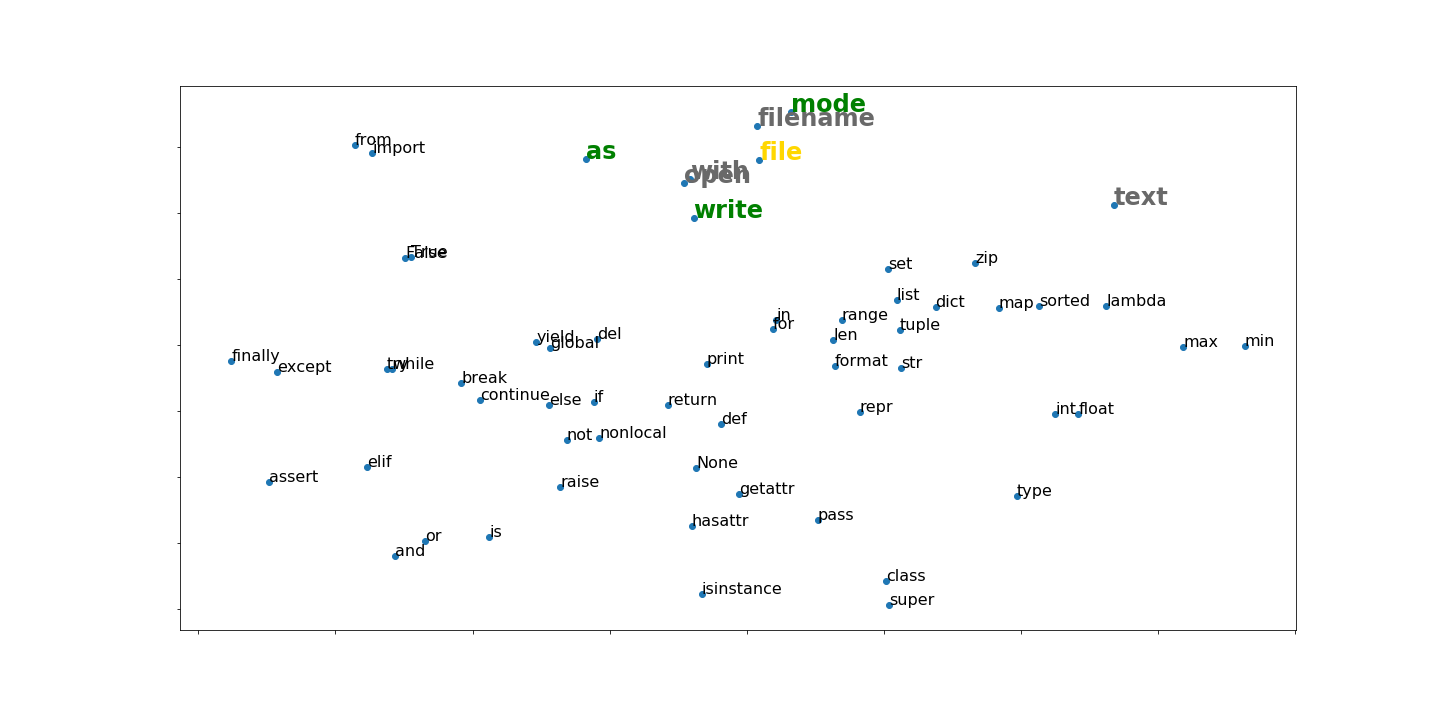
\includegraphics[width=1\textwidth]{figuras/cap-trabalhos-relacionados/code-tsne-output.png}
\caption{Representação em 2D do vetor de representação distribuída de trechos de código-fonte. Imagem gerada através da ferramenta t-SNE. E o vetor de representação distribuída foi criado a partir da amostra de trechos de código-fonte em Python disponibilizada por \cite{yao-2018}. Vetor criado utilizando o \textit{word2vec} com o algoritmo \textit{skip-gram} e o parâmetro \textit{window} com o valor $5$.}
\label{fig:tsne-code-snippet-python}
\end{figure}

\section{Arquiteturas}

Para este estudo, comparamos as arquiteturas bi-LSTM com CNN, CNN com uma arquitetura de referência \textit{Embedding}. A arquitetura \textit{Embedding} combina os vetores de representação distribuída de cada palavra através de uma camada \textit{max pool}. As outras arquiteturas seguem a descrição feita no capítulo abordagem \todo{citar o capítulo}.

Abaixo tem as figuras ilustrativas das arquiteturas utilizadas:

\todo{adicionar as figuras do artigo}

Conforme as figuras, todas as arquiteturas utilizam uma camada \textit{max pool} e, ao final, calculam a similaridade atravás da função \textit{cosine}.
Não realizamos otimização ou tuning dos hiper-parâmetros dos modelos. Utilizamos os mesmos hiper-parâmetros propostos por \cite{tan-lstm-qa}. Exceto o hiper-parâmetro filtro da camada CNN, neste caso utilizamos o valor $100$, pois o valor $1000$ proposto por \cite{tan-lstm-qa} aumentou a capacidade do modelo e estava causando \textit{overfitting}.

Para a função de perda \textit{hinge}, utilizamos o valor $0,009$ proposto por \cite{feng-2015} para a margem. Em relação a dimensão do vetor de representação distribuída das palavras (\textit{word embedding}), utilizamos o valor $100$.


%% ------------------------------------------------------------------------- %%
\section{Resultados preliminares}

Os resultados preliminares foram coletados a partir da avaliação dos modelos na amostra \emph{EVAL}. O valor final MRR é a média obtida após avaliar o modelo durante 20 iterações. 

\begin{table}[h]
\centering
\begin{tabular}{ p{3cm} p{3cm} }
 \hline
 \textbf{Modelos} & \textbf{Resultados (MRR)}\\
 \hline
 Embedding & $0,52 \pm 0,01$\\
 
 CNN & $0,58 \pm 0,01 $ \\
 
 \textbf{bi-LSTM-CNN} & $\bm{0,60} \pm \bm{0,02}$\\
 \hline
\end{tabular}
\caption{Resultado preliminar do modelo bi-LSTM-CNN proposto em comparação a outros dois modelos (CNN e Embedding). Estes resultados foram obtidos a partir da amostra EVAL.}
\label{table:resultados-preliminares}
\end{table}

Conforme a tabela~\ref{table:resultados-preliminares}, tanto o \emph{CNN} quanto o bi-LSTM com CNN obtiveram resultados próximos. O\emph{CNN} obteve um resultado relativamente menor, mas o seu tempo de duração de treinamento é de apenas 6s. Enquanto o treinamento do bi-LSTM durou cerca de 48 minutos. Tanto o treinamento quanto a avaliação foram executadas na plataforma Colab \todo{criar glossário} do Google. No momento de treinamento e coleta dos resultados, a execução foi feita em uma máquina virtual com acesso a uma vGPU \todo{criar acronimo} Tesla K80.

Para entender um pouco melhor o resultado da média harmônica MRR, a figura abaixo exibe as posições da primeira ocorrência do trecho de código-fonte encontradas durante a avaliação dos modelos.

\todo{acrescentar a figura do PPT do VEM}

Tanto o bi-LSTM com CNN quanto CNN conseguiram classificar os trechos de código-fonte entre as 3 (três) primeiras posições em 75\% dos casos. O modelo bi-LSTM com CNN obteve uma precisão TOP-1 de 51\%, i.e., em mais da metade das vezes, o trecho de código-fonte relevante ficou na primeira posição. 





